% =====================================================================
% Notebook 3 (Flood model), second half, round 2: cells 42 to 61
% =====================================================================
\begingroup\emergencystretch=6em

\subsection{Section 5: Capsule network and severity ratings (cells 42 to 44)}
\textbf{Where.} Cell 42 is markdown, cells 43 and 44 are code and print nothing. From here every $64\times64$ tile gets one of four ratings for 30 minutes ahead. The rating is the share of the tile's normally dry land (rivers and lakes left out) under more than 30 cm of water, with limits \cd{SEVERITY\_LIMITS = [0.05, 0.15, 0.30]}. The markdown says ``above 30\%'' for Severe, but \cd{np.digitize} puts exactly 30\% into Severe, as the report does.

\begin{center}
\small
\begin{tabular}{|l|c|c|c|c|}
\hline
\rowcolor{black!12} \hd{Rating} & None (0) & Minor (1) & Moderate (2) & Severe (3)\\ \hline
Dry land under more than 30 cm & below 5\% & 5\% to 15\% & 15\% to 30\% & 30\% or more\\ \hline
\end{tabular}
\end{center}
\textbf{The idea.} The network sits on top of Model A and reuses its CNN and ConvLSTM, frozen. Each rating gets its own list of 16 numbers, a \term{capsule}. The \textbf{length} of the list is how sure the network is, and the answer is the rating with the longest list. The notebook gives no reason for 16.

\paragraph{Squash (cell 43, lines 3 to 4).}
\codelines{model_c43}{3}{4}
Line 3 squares every number and adds them along the last axis (\cd{keepdims=True} keeps that axis), giving $L$, the squared length. Line 4 makes new vector $=\frac{L}{1+L}\times\frac{\text{vector}}{\sqrt L}$: the direction scaled to length 1, times a new length $L/(1+L)$. The \cd{1e-7} avoids dividing by zero. A short vector stays short and a long one gets close to 1 but never reaches it, so every length is between 0 and 1 and reads as a confidence. Examples: $(0.3,0.4)$ has length 0.5 and becomes length 0.2. $(3,4)$ has length 5 and becomes 0.962. $(30,40)$ has length 50 and becomes 0.9996. Lines 7 to 10 only wrap \cd{squash} in a layer class \cd{Squash}.

\paragraph{ClassCapsules: weights and routing by agreement.}
\codelines{model_c43}{26}{30}
\cd{build} runs once, when the input (b, 256, 8) is known: 256 small (primary) capsules of 8 numbers. \cd{add\_weight} makes the learnable numbers, shape $(256,4,16,8)$, a $16\times8$ matrix for every (small capsule, class) pair, $256\times4\times128=131{,}072$ weights (our own count), starting as small random numbers (\cd{stddev=0.05}). A matrix turns 8 numbers into 16, a \emph{vote}.
\codelines{model_c43}{32}{50}
In the einsum letters \cd{b} is batch, \cd{p} small capsule (256), \cd{c} class (4), \cd{o} number inside a class capsule (16), \cd{i} number inside a small capsule (8). A letter left of \cd{->} but missing on the right is added up.
\begin{itemize}
\item \textbf{Lines 32 to 34.} \cd{"pcoi,bpi->bpco"}: \textbf{each of the 256 small capsules votes for each of the 4 classes}, 16 numbers per vote, shape (b, 256, 4, 16).
\item \textbf{Lines 36 to 41.} \cd{routing\_scores} starts as zeros (b, 256, 4). The loop runs 3 times. \cd{softmax} over the classes turns each small capsule's 4 scores into the \term{coupling}, positive shares adding to 1. Scores $(0,0,0,0)$ give 0.25 each, $(2,0,0,0)$ give $(0.711,0.096,0.096,0.096)$.
\item \textbf{Lines 43 to 44.} \cd{"bpc,bpco->bco"}: each vote times its coupling, added over the 256, gives 4 class capsules of 16 numbers, then \cd{squash}.
\item \textbf{Lines 46 to 48.} If not the last round, \cd{"bpco,bco->bpc"} takes the dot product of each vote with the class capsule just made (big positive means ``my vote agrees'') and \emph{adds} it to \cd{routing\_scores}, so next round that small capsule sends more of its vote to the classes it agrees with. Line 50 returns the last round.
\end{itemize}
Think of 256 reporters writing for four judges. At first each report counts a quarter for each judge. Then each reporter sends more to the judges whose note agrees with his. The notebook does not say why 3 rounds. We think it follows the capsule paper (Sabour and colleagues, cited in the report). This is general reasoning, not tested here.

\paragraph{CapsuleLength and the margin loss.}
\codelines{model_c43}{53}{63}
\cd{CapsuleLength} squares the 16 numbers, adds them (the 16 disappear) and takes the root: input (b, 4, 16), output (b, 4), \textbf{four lengths per tile between 0 and 1}, the network's output. In \cd{margin\_loss}, \cd{true\_classes} is one-hot, for example $(0,0,1,0)$ for Moderate, and the comment gives the aim: right class above 0.9, others below 0.1. Line 61: \cd{relu(0.9 - lengths)} is how far the right length is below 0.9, squared. Line 62: \cd{relu(lengths - 0.1)} is how far a wrong length is above 0.1, squared, times 0.5 so wrong classes count half (in the capsule paper the reason is that absent classes should not shrink all lengths early on, general reasoning). Line 63 adds the four penalties. With true class Moderate, lengths $(0.05,0.05,0.95,0.05)$ cost 0. Lengths $(0.05,0.30,0.80,0.10)$ cost $0.1^2+0.5\times0.2^2=0.03$. Lengths $(0.90,0.10,0.10,0.10)$ cost $0.8^2+0.5\times0.8^2=0.96$.

\qq{What is routing by agreement, and why is the length the confidence?}{Small capsules vote for every class and votes that match the result get more weight in the next of 3 rounds, while squash keeps lengths below 1 and the margin loss pushes the right class above 0.9.}{}

\paragraph{Building the network on Model A (cell 44).}
\codelines{model_c44}{11}{15}
Line 11: \cd{forecaster.get\_layer("memory").output} is the output of the ConvLSTM layer named \cd{"memory"}, and \cd{keras.Model(input, output)} makes \cd{encoder}, \textbf{Model A cut off after the ConvLSTM}, with the weights Model A already learned. Output: 32 memory maps of $64\times64$. Line 12, \cd{encoder.trainable = False}, \textbf{freezes} it. Lines 14 to 15 pass a new input through it to get \cd{memory} (b, 64, 64, 32).

\textbf{Why frozen?} The notebook only says ``frozen''. Our reading is that Model A has already learned how water moves from 4,000 tiles, so the new layers only learn the rating and Model A's forecast stays unchanged. One sign agrees: the optimizer warning (cell 46) says the capsule optimizer has 16 variables, and Adam keeps 2 counters plus 2 per trained array, so $16=2+2\times7$ is 7 trained arrays, the new layers (3 convolutions with kernel and bias, plus the vote weights). Model A shows 24, $2+2\times11$. This is our own check.
\codelines{model_c44}{17}{24}
Lines 17 to 19: two convolutions with 32 filters of $5\times5$, \cd{strides=2} halves the map ($64\to32\to16$), \cd{padding="same"} keeps only the stride changing the size. The notebook gives no reason for $5\times5$. Generally a stride-2 convolution shrinks the map and learns what to keep, and $5\times5$ sees more neighbours than $3\times3$. Line 22: $4\times8=32$ filters of $3\times3$, stride 2, no activation, giving $8\times8$ positions. Line 23: \cd{Reshape((8 * 8 * 4, 8))} cuts the 32 numbers at each position into 4 pieces of 8, so $64\times4=256$ small capsules. Line 24 squashes them (\term{primary capsules}). Lines 27 to 33 add \cd{ClassCapsules(4, 16, ...)} and \cd{CapsuleLength}. \cd{model} gives four lengths. \cd{grad\_cam\_model} has the same layers with two outputs, the memory maps and the lengths, because Grad-CAM needs the memory. The 8 comes from \cd{TILE\_SIZE // 8}, three halvings.

\begin{center}
\small
\begin{tabular}{|l|l|l|}
\hline
\rowcolor{black!12} \hd{Step} & \hd{Shape} & \hd{Meaning}\\ \hline
Input tiles & (b, 4, 64, 64, 3) & 4 maps, 3 layers\\ \hline
Frozen CNN + ConvLSTM & (b, 64, 64, 32) & 32 memory maps\\ \hline
Conv $5\times5$ s2 twice, conv $3\times3$ s2 & (b, 32, 32, 32), (b, 16, 16, 32), (b, 8, 8, 32) & map shrinks\\ \hline
Reshape + Squash & (b, 256, 8) & 256 small capsules\\ \hline
ClassCapsules, CapsuleLength & (b, 4, 16), (b, 4) & class capsules, four lengths\\ \hline
\end{tabular}
\end{center}

% ---------------------------------------------------------------------
\subsection{Labels, class weights, loading and test tiles (cells 45 to 47)}
\textbf{Cell 45} (\cd{tile\_labels}) gives every tile its correct rating.
\codelines{model_c45}{4}{8}
\cd{positions[number]} is (time, top row, left column), \cd{region["dry\_land"][...]} cuts the dry-land mask of that piece, \cd{targets[number][:, :, 0]} is the depth 30 minutes later, \cd{flooded\_share} gives the share of dry land deeper than 30 cm and \cd{severity\_class} turns it into 0 to 3. Lines 11 to 22 loop over both scales and count tiles per class with \cd{np.bincount(labels, minlength=4)}.

\begin{center}
\small
\begin{tabular}{|l|r|r|r|r|r|r|r|r|}
\hline
\rowcolor{black!12} & \multicolumn{4}{c|}{\hd{Training tiles (sum 4,000)}} & \multicolumn{4}{c|}{\hd{Class weight (our calculation)}}\\ \hline
\rowcolor{black!12} \hd{Model} & None & Minor & Mod. & Severe & None & Minor & Mod. & Severe\\ \hline
30m & 1942 & 1619 & 359 & 80 & 0.515 & 0.618 & 2.786 & 12.500\\ \hline
480m & 234 & 562 & 1318 & 1886 & 4.274 & 1.779 & 0.759 & 0.530\\ \hline
\end{tabular}
\end{center}
In Australia (30 m) only 80 tiles (2\%) are Severe. In Pakistan (480 m) 1,886 (about 47\%) are, because a 480 m tile covers about 30 km against about 2 km at 30 m (report).

\textbf{Cell 46} builds the capsule network on the trained Model A of each scale and loads saved weights. Nothing was trained in this run (\cd{TRAIN\_NEW = False}).
\codelines{model_c46}{10}{11}
\codelines{model_c46}{16}{21}
Lines 10 to 11: Adam with step 0.001, \cd{loss=margin\_loss} and an accuracy metric. Lines 16 to 19, \textbf{class weights}: \cd{len(labels) / (4 * counts)} is $4000/(4\times\text{count})$, and \cd{class\_weights[data["train\_labels"]]} gives each tile its class weight (used as \cd{sample\_weight}), so rare classes count more. Each class then has equal total weight, for example $80\times12.5=1000=1942\times0.515$. Line 21: \cd{EarlyStopping(patience=5, restore\_best\_weights=True)} stops after 5 epochs without a better checking loss and restores the best weights. The unused training branch is \cd{model.fit} with one-hot labels, \cd{epochs=30}, \cd{batch\_size=32}. The cell prints the loading message and the harmless optimizer warning (2 variables against 16 saved: the file also holds Adam's training memory, not needed for prediction). The same warning appeared for Models A and B.

\textbf{Cell 47} cuts \cd{TEST\_TILES = 1000} random test tiles per flood (the last 15\% in time of the training floods, and the whole never-seen UK and Mozambique floods). \cd{predict} gives lengths (1000, 4) and Model A's forecast (1000, 64, 64, 1), and \cd{np.argmax(lengths, axis=1)} is the \textbf{answer}, the longest capsule.
\begin{carefulbox}
The 1,000 tiles are not independent. From map sizes we worked out the (time, tile) pairs (not printed): Australia $256\times73=18{,}688$, UK $8\times140=1{,}120$, Pakistan $72\times101=7{,}272$, Mozambique $4\times284=1{,}136$. In the UK nearly every pair is used and neighbours 30 minutes apart look almost the same.
\end{carefulbox}
\qq{Why class weights?}{The 30 m model has 1,942 None tiles and only 80 Severe, so Severe gets weight 12.5 and None 0.515, otherwise answering None would score well and teach little.}{}
\qq{Did the capsule network train in this run?}{No, weights were loaded from Drive, the training code is up to 30 epochs with early stopping after 5 without improvement.}{}

% ---------------------------------------------------------------------
\subsection{The confusion matrices (cell 48)}
\codelines{model_c48}{6}{10}
Line 6: \cd{confusion\_matrix(true, answer, labels=range(4))} counts tiles, row $i$ column $j$ being true class $i$ answered $j$. Line 7 draws it (darker blue is more tiles). Lines 9 to 10: \cd{np.mean(labels == capsule\_classes)} is the accuracy in the title. The other lines make 4 plots and save \cd{05\_capsule\_confusion.png}.

\nbfig{model_c48_8.jpg}{0.55}{Capsule confusion matrices on 1,000 test tiles per flood (Australia, UK, Pakistan, Mozambique). Rows true rating, columns the answer, accuracy in each title.}
\textbf{Say this:} the diagonal holds the correct answers and each matrix adds to 1,000. The overlapping y-label is only a layout problem.

\begin{center}
\small
\begin{tabular}{|l|c|c|c|c|l|}
\hline
\rowcolor{black!12} \hd{Flood} & True None & Minor & Moderate & Severe & \hd{Diagonal}\\ \hline
Australia (30 m) & 94 & 134 & 318 & 454 & 22+65+125+397 = 609\\ \hline
UK (30 m) & 189 & 618 & 193 & 0 & 126+297+77+0 = 500\\ \hline
Pakistan (480 m) & 56 & 79 & 167 & 698 & 41+48+125+660 = 874\\ \hline
Mozambique (480 m) & 290 & 375 & 201 & 134 & 161+285+89+100 = 635\\ \hline
\end{tabular}
\end{center}
Titles: 60.9\%, 50.0\%, 87.4\%, 63.5\%.
\begin{itemize}
\item \textbf{Pakistan.} 660 of 698 truly Severe tiles (94.6\%) were found. But 698 of 1,000 are Severe, so always answering ``Severe'' gives 69.8\% and the 87.4\% is less impressive than it looks.
\item \textbf{UK.} The Severe row is all zeros because no UK test tile is truly Severe. 101 tiles were wrongly answered Severe. Of the 500 wrong answers, 479 are one class away.
\item \textbf{Australia.} 649 tiles were answered Severe but only 454 are truly Severe. The 49 truly None answered Severe are unexplained (rule 1 also fires 49 times there).
\item \textbf{Mozambique.} It never answers Severe for a tile below Moderate.
\end{itemize}
\qq{How good is the capsule network?}{Right for 50\% to 87\% of tiles, most mistakes are one class away, and Pakistan's high number mostly reflects that most of its tiles are Severe.}{The 30 m and 480 m accuracies should not be compared because the tiles cover different areas.}

% =====================================================================
\subsection{Section 6: Grad-CAM (cells 49 to 52)}
Grad-CAM (explainable AI, Chapter~\ref{ch:gradcam}) draws a heat map of which places mattered most for one number, in four steps. (1) Pick one number: for Model A the total predicted water, for the capsule network the length of the chosen class capsule. (2) Gradient: for each square of each of the 32 ConvLSTM memory maps, how much the number changes if that value goes up a little. (3) One weight per memory map: its gradient averaged over the map. (4) Multiply each map by its weight, add the 32, keep only the positive part.
\codelines{model_c50}{5}{10}
Line 5: \cd{tf.GradientTape()} records everything so gradients can be worked out later. Line 6: the model returns \cd{memory} (1, height, width, 32) and \cd{output}, with \cd{training=False}. Lines 7 to 10: with no class number \cd{tf.reduce\_sum(output)} is the total forecast, otherwise \cd{output[0, class\_number]} is that capsule's length.
\codelines{model_c50}{12}{22}
Lines 12 to 13: \cd{tape.gradient(explained, memory)}, same shape as \cd{memory}. Lines 15 to 16: \cd{reduce\_mean(..., axis=(1, 2))} gives (1, 32), one weight per map. Lines 18 to 19: \cd{channel\_weights[:, None, None, :]} makes shape (1, 1, 1, 32) so each map is multiplied by its own weight, \cd{reduce\_sum(axis=-1)} adds the 32, \cd{relu} sets negatives to 0, \cd{[0].numpy()} takes the single item. Lines 21 to 22 divide by \cd{heatmap.max()} so the brightest is 1 (\cd{1e-8} avoids division by zero). The heat map has the input's size because the memory maps do, so no resizing is needed.

\paragraph{The 256 window.}
\codelines{model_c50}{41}{51}
For big maps the notebook zooms into a window of at most $256\times256$ (\cd{GRAD\_CAM\_WINDOW = 256} on line 30). The cell says a whole map does not fit in GPU memory. We think it is because Grad-CAM keeps all 32 memory maps and gradients at once. Lines 41 to 43 give the window size, at most 256 each way. Lines 45 to 47: \cd{uniform\_filter(change, size=31)} averages the true change over $31\times31$ squares, so the busiest spot is a busy \emph{area}. Line 48: \cd{np.argmax} and \cd{np.unravel\_index} give its (row, column). Lines 50 to 51: the window starts at centre minus half its size and \cd{np.clip(value, 0, rows - height)} keeps it inside the map. Windows (our calculation): Australia $256\times256$, UK $170\times256$, Pakistan $256\times256$, Mozambique $151\times138$ whole map.

\textbf{Cell 51} runs Model A's Grad-CAM for each flood. It builds Model A at window size with \cd{build\_forecaster(height, width)}, copies the trained weights in with \cd{set\_weights(...get\_weights())} (convolutions work at any size), and calls \cd{grad\_cam} with no class number.
\codelines{model_c51}{15}{16}
The drawing lines clip colours at the 99th and 99.5th percentiles and draw, per flood, water now, predicted change (blue rising, red falling) and the heat map in \cd{inferno} (purple little, yellow most) at 60\% opacity over grey ground height. \textbf{Cell 52} does the capsule network on the 4 most flooded tiles (\cd{np.argsort(shares)[-4:]}) of the UK and Mozambique, with the network's \emph{chosen} class (so it explains the capsule the network chose, not the correct one), the input depth (0 to 2 m) above and the heat below.

\begin{figure}[!htbp]
\centering
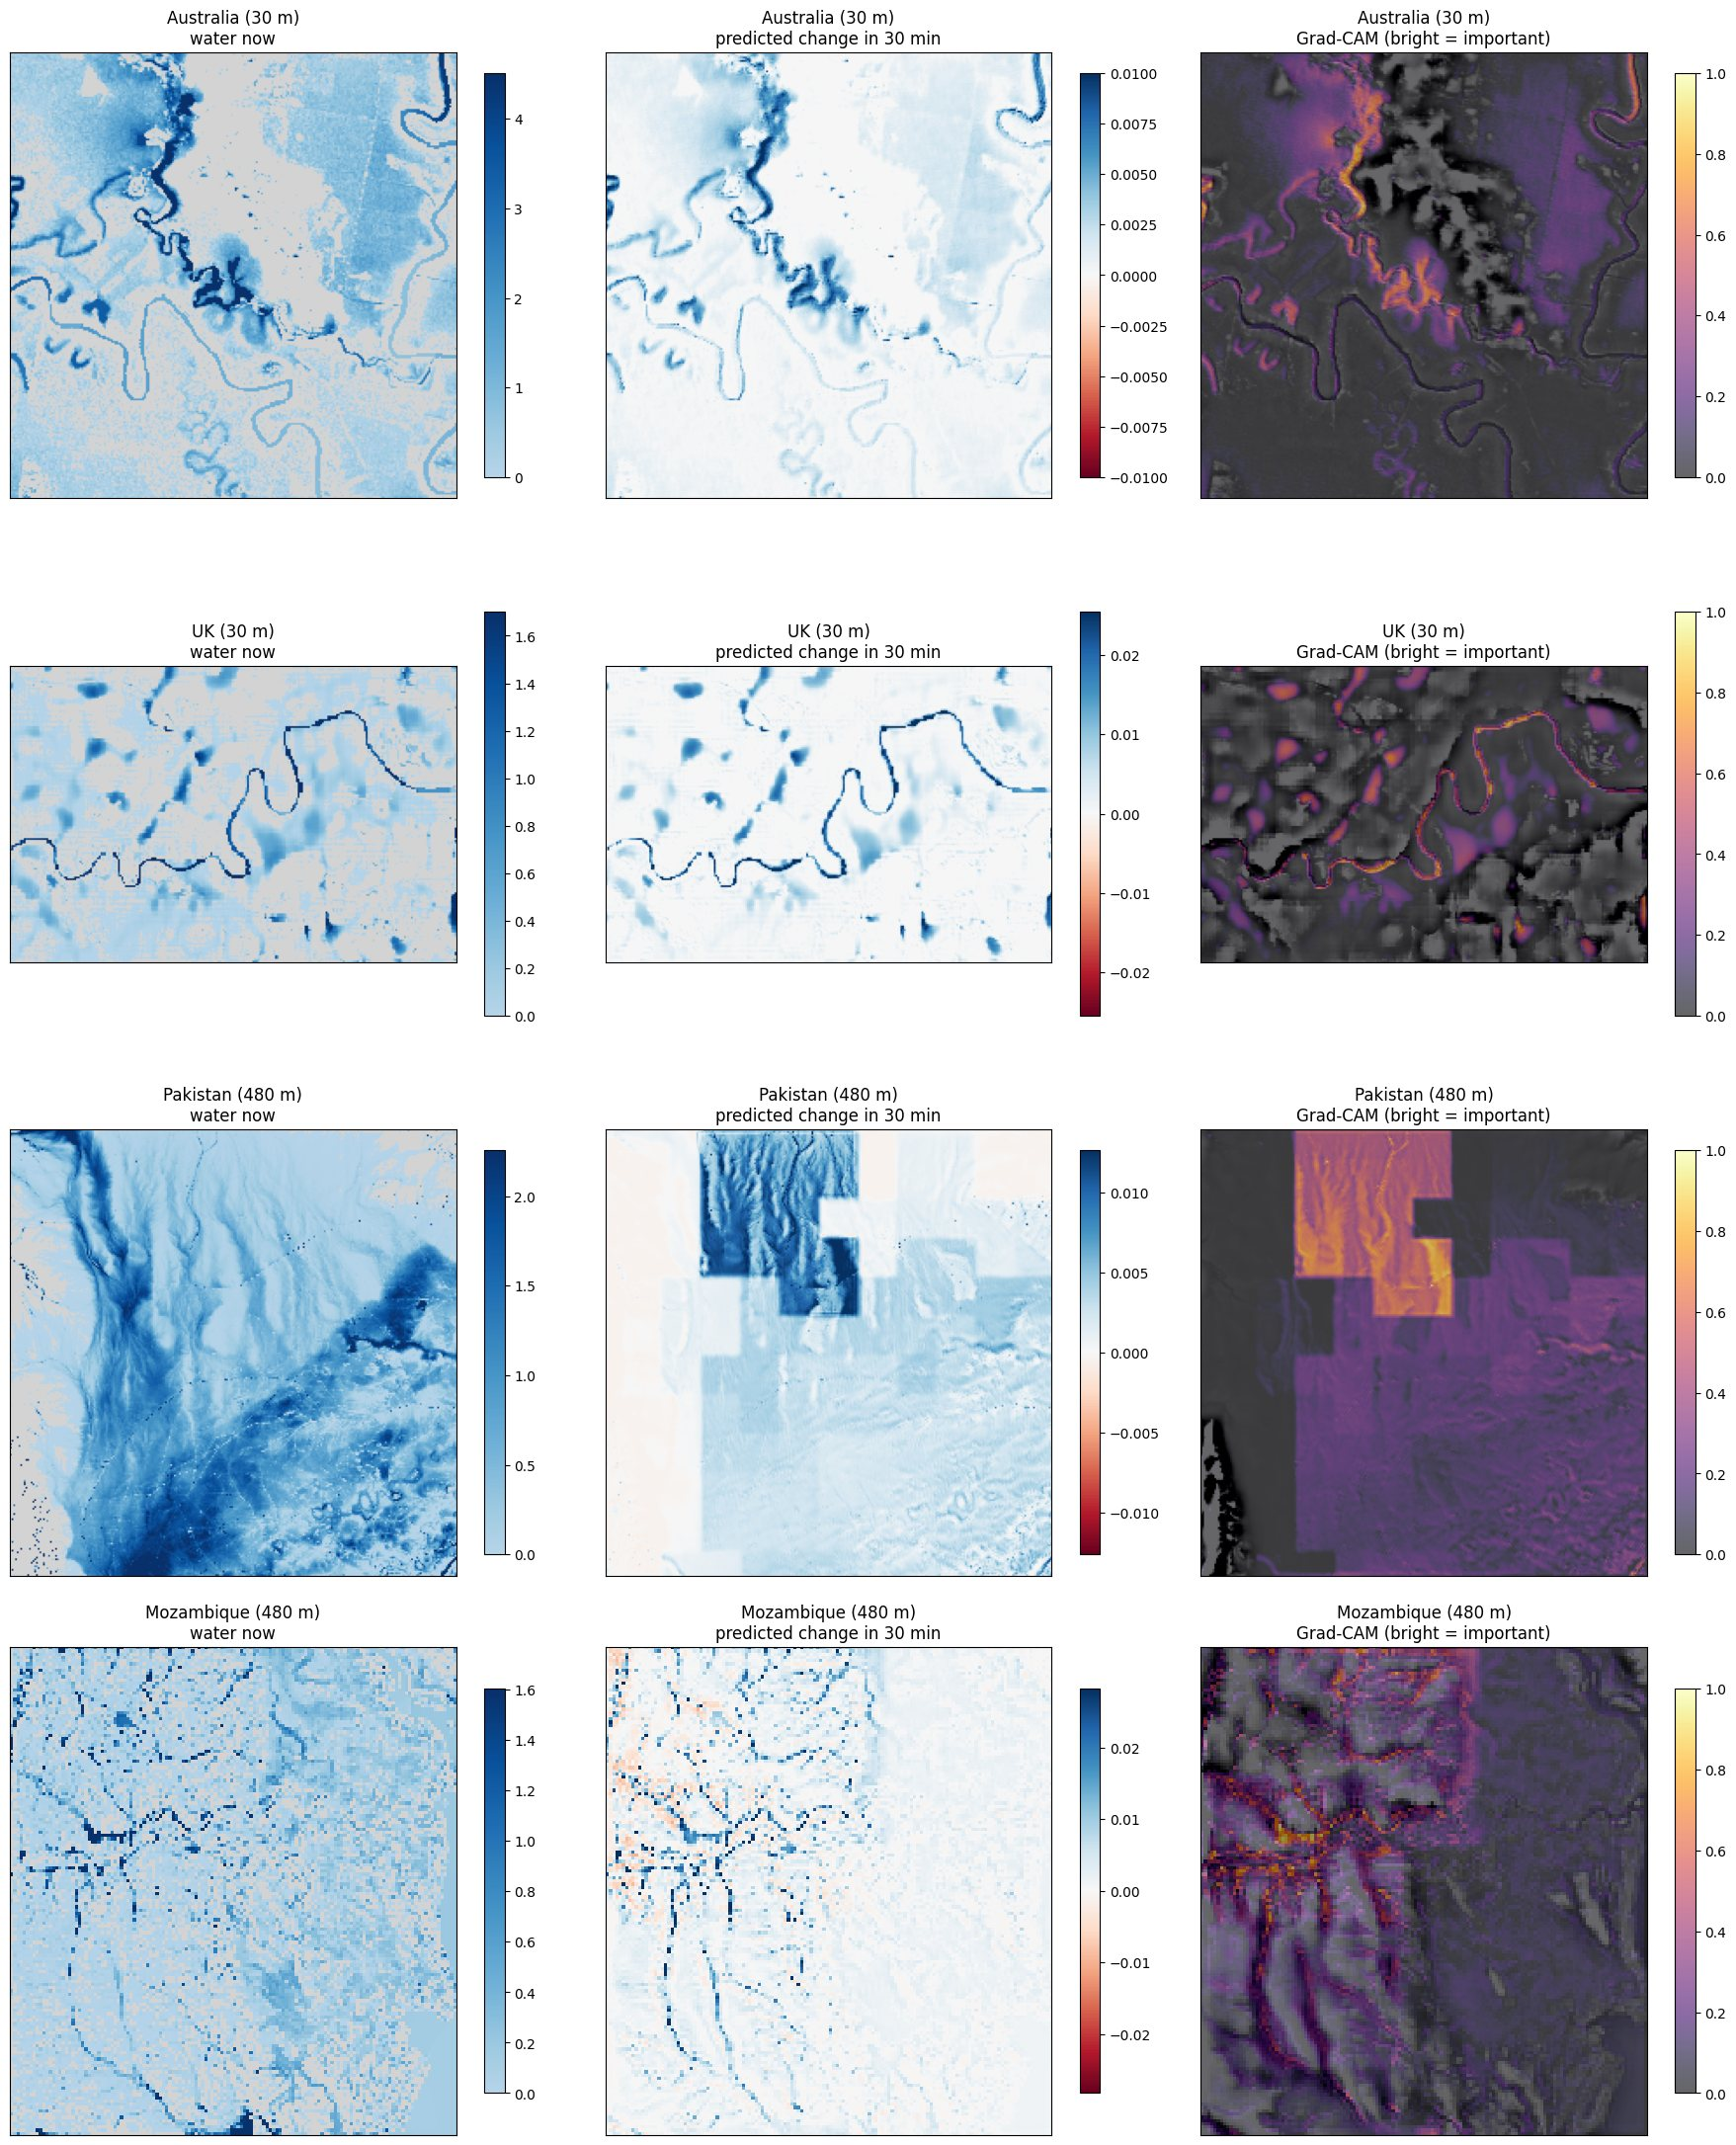
\includegraphics[width=0.4\linewidth]{nbfigs/model_c51_9.jpg}\hspace{0.01\linewidth}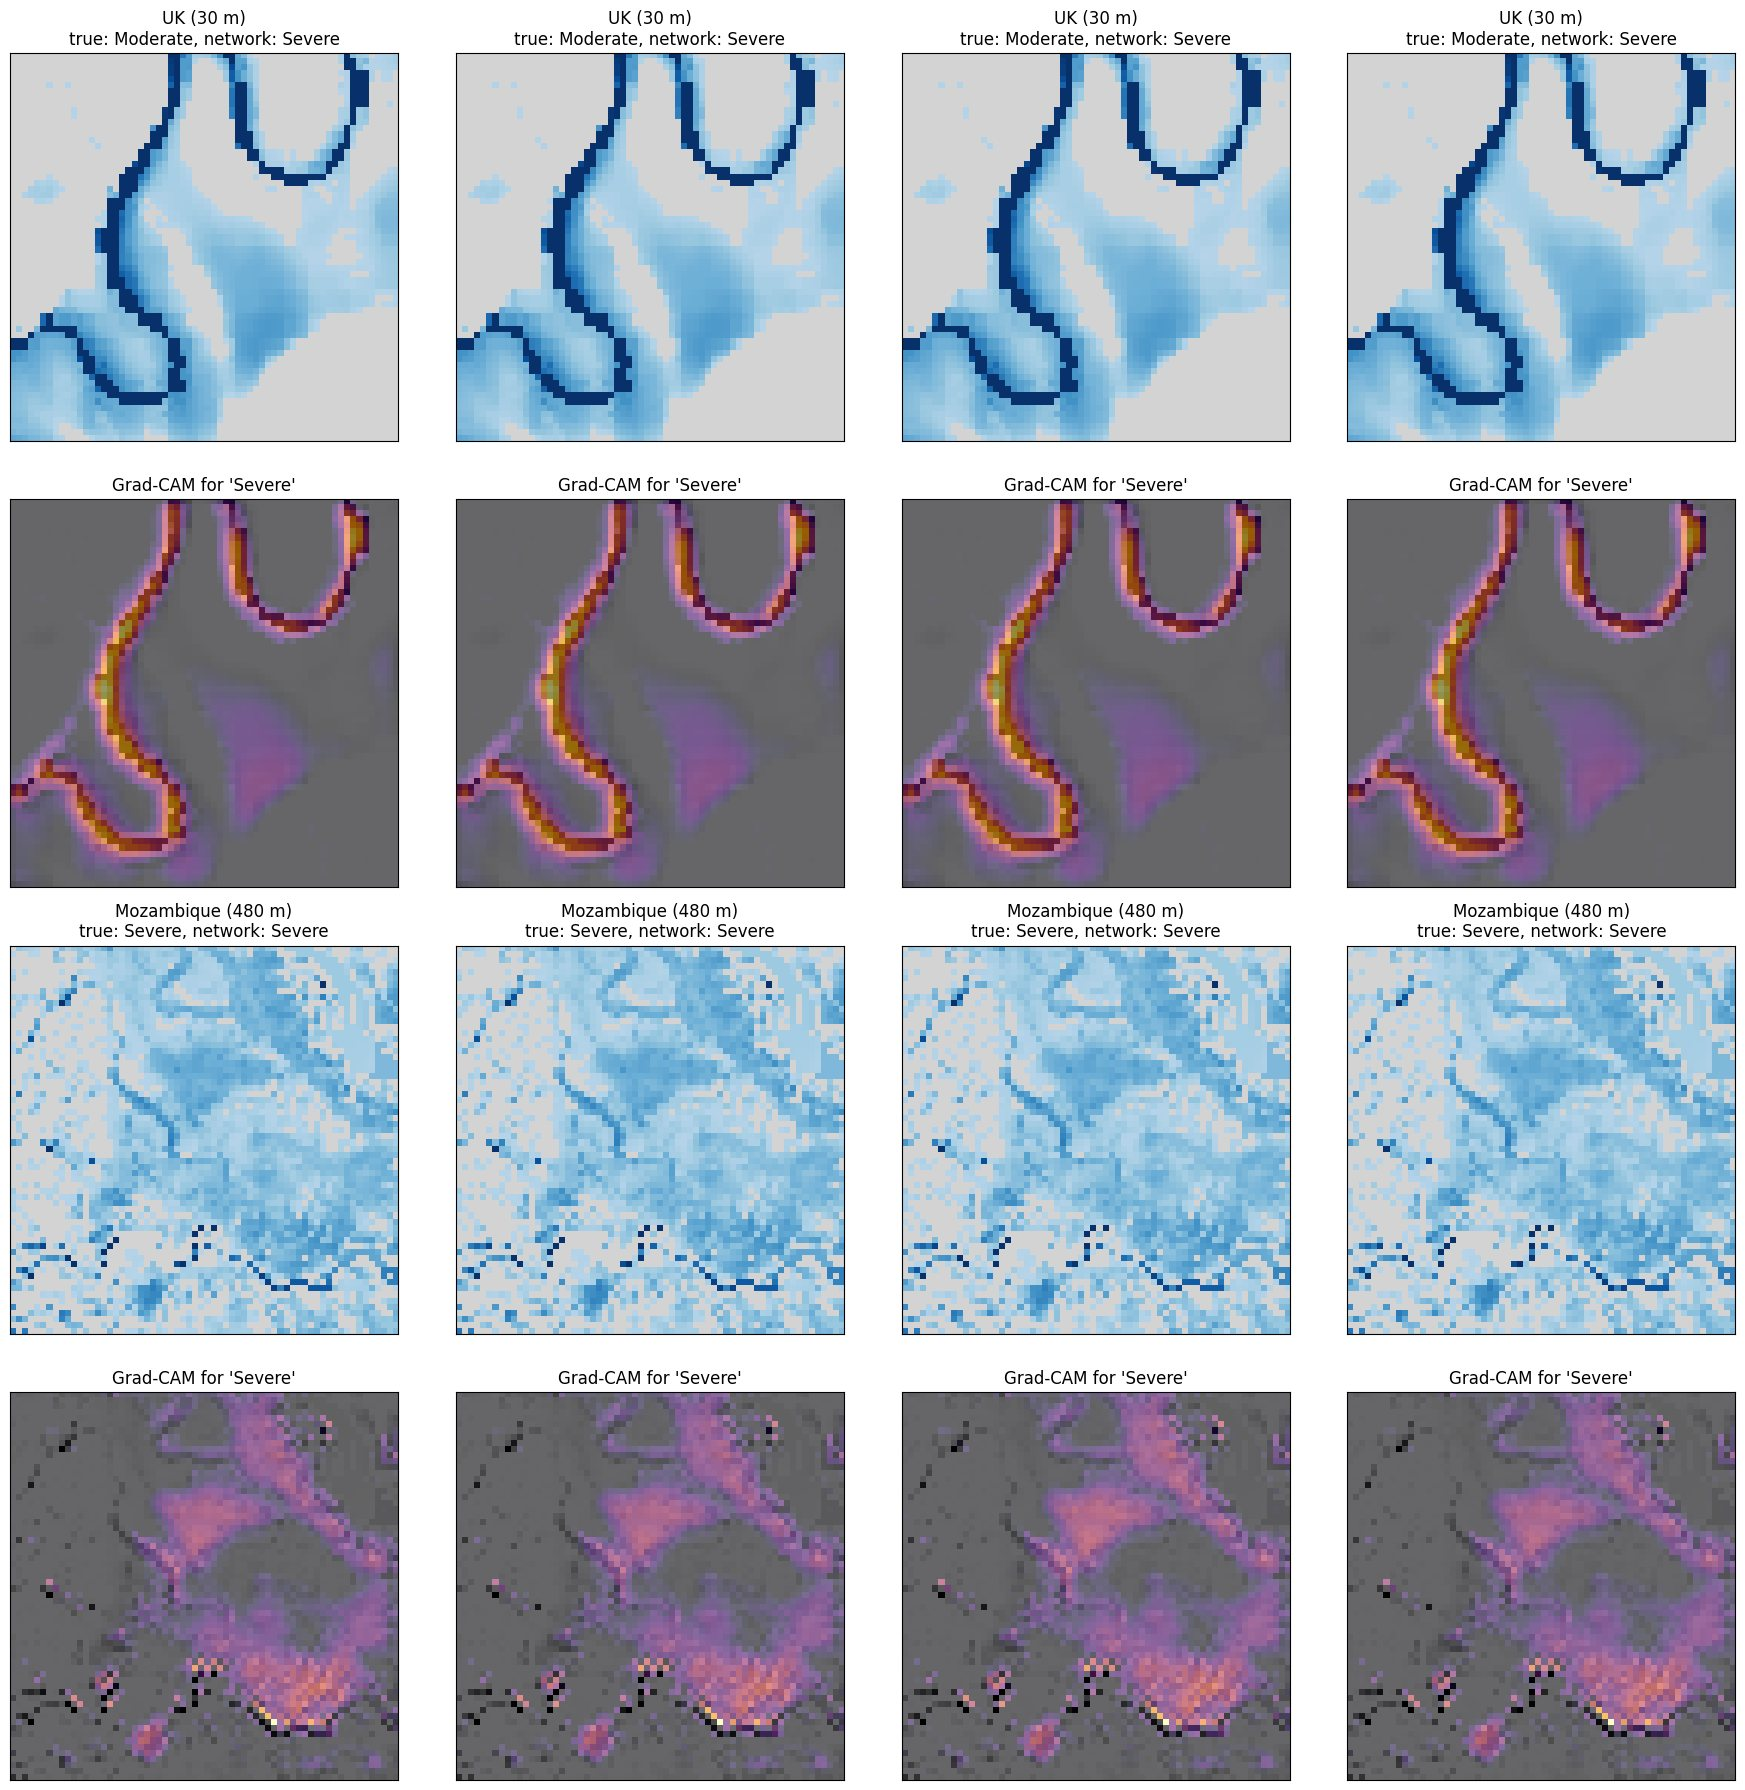
\includegraphics[width=0.3\linewidth]{nbfigs/model_c52_10.jpg}
\caption{Left: Grad-CAM of Model A (rows Australia, UK, Pakistan, Mozambique, columns water now in m, predicted change in m, heat 0 to 1). Right: capsule network (rows 1 and 2 UK, rows 3 and 4 Mozambique, water now above its heat map).}
\end{figure}
\textbf{Say this (Model A):} the heat is brightest where the predicted change is largest: the deep channel in Australia, thin lines along bends in the UK, square blocks in Pakistan (we think from blocks of heavy rain in the data, their straight edges are not how water behaves) and the drainage lines in Mozambique. It shows where the number is most sensitive, not that the forecast is right. The predicted change is tiny, about 1 to 3 cm in 30 minutes. The report adds that in the earlier laptop study deleting the top 10\% of the heat map changed the forecast more than random cells in 84\% to 92\% of windows, not run in this notebook.

\textbf{Say this (capsule):} in the UK all four tiles read ``true Moderate, network Severe'' with heat on the deep channel. In Mozambique all four read ``Severe, Severe'' with spread-out heat. The four columns look alike and are very probably one tile at neighbouring times (we think). The report says the capsule heat maps were weak (top cells beat two control sets in only 55\% of windows, two seeds agreed with rank correlation 0.17), so they are illustrations, not proof.

\qq{What number does each Grad-CAM explain, and why average gradients and use ReLU?}{Model A: the total predicted water of the window. Capsule network: the length of the chosen class capsule. Averaging gives one weight per memory map and ReLU keeps only places that push the number up, the standard recipe.}{}

% =====================================================================
\subsection{Section 7: Written rules, the NeuroSymbolic part (cells 53 to 58)}
\term{NeuroSymbolic AI} joins a network that learns patterns (Model A, capsule network) with rules people write down (these three plus the water-balance rule of Section 3a). The written reason of each decision is the explainable part.

\begin{center}
\small
\begin{tabularx}{\linewidth}{|>{\bfseries}l|Y|Y|Y|}
\hline
\rowcolor{black!12} \hd{Rule} & \hd{When it applies} & \hd{What it does} & \hd{Why (our reading)}\\ \hline
1. No water, no flood & under 1\% of dry land flooded now and in the forecast & answer None & almost nothing wet now and soon makes a higher rating implausible\\ \hline
2. Rising water & forecast flooding at least as much as now, more than 1 mm/h rain in the last hour, network class below current class & answer is the current class & flooding not shrinking during rain should not be rated below what is already there\\ \hline
3. Agree with the forecast & network more than one class from the forecast map's class & answer is the forecast map's class & the forecast map is measured from depths, the network is a guess\\ \hline
\end{tabularx}
\end{center}
The notebook gives no written reasons for the limits (1\% and 1 mm/h), so the last column is our reading.
\codelines{model_c54}{12}{25}
\cd{ALMOST\_DRY\_SHARE = 0.01} and \cd{RAIN\_RULE\_MM\_PER\_HOUR = 1.0} are the limits, and \cd{severity\_class} turns the two shares into \cd{now\_class} and \cd{forecast\_class}. Lines 12 to 14, rule 1: \cd{return 0, "Rule 1: ..."} ends the function at once. Lines 16 to 18, rule 2: three conditions joined by \cd{and}, and \cd{network\_class < now\_class} means rule 2 can only \emph{raise} the answer. Lines 20 to 23, rule 3: \cd{abs(network\_class - forecast\_class) > 1}. Line 25: no rule fired, ``No rule needed''. \textbf{Order matters}: the first rule that applies decides.

\textbf{Cell 55} runs it for every test tile. Share now and share forecast come from the last depth map and Model A's forecast tile. Rain last hour is \cd{data["inputs"][tile, -2:, :, :, 1].mean() * RAIN\_SCALE}: the last two maps (two 30-minute steps), averaged, times 10 to undo the division when the input was built, giving mm per hour.

\textbf{Cell 56} (accuracy with and without rules, saved as \cd{07\_neurosymbolic\_accuracy.csv}) and \textbf{cell 57} (which rule decided, by cutting each reason at the colon):
\begin{center}
\small
\begin{tabularx}{\linewidth}{|l|Y|Y|Y|Y|r|r|r|r|}
\hline
\rowcolor{black!12} \hd{Flood} & \hd{Capsule alone} & \hd{Forecast-map class} & \hd{Capsule + rules} & \hd{Changed} & \hd{None needed} & \hd{R1} & \hd{R2} & \hd{R3}\\ \hline
Australia (30 m) & 60.9\% & 99.8\% & 67.9\% & 7.0\% & 930 & 49 & 0 & 21\\ \hline
UK (30 m) & 50.0\% & 99.1\% & 56.1\% & 6.1\% & 939 & 0 & 40 & 21\\ \hline
Pakistan (480 m) & 87.4\% & 99.9\% & 89.1\% & 1.7\% & 983 & 0 & 7 & 10\\ \hline
Mozambique (480 m) & 63.5\% & 99.5\% & 70.7\% & 7.2\% & 824 & 134 & 42 & 0\\ \hline
\end{tabularx}
\end{center}
The gains (7.0, 6.1, 1.7, 7.2 points) equal the changed decisions (70, 61, 17, 72 tiles), and a change adds at most one correct tile, so every changed decision turned a wrong answer into a right one (our calculation). A rule that fired did not always change the answer: in Mozambique 134 tiles got rule 1 but rule 1 changed only 30 answers, in 104 the network already said None (our calculation). \textbf{Why the forecast map scores 99\%:} the rating in 30 minutes is almost the rating now because water changes slowly, so the class read off the forecast map is nearly always right (the report says the classifier adds little). Pakistan's 87.4\% is flattered by the 69.8\% baseline.

\textbf{Cell 58} shows ten example decisions (UK and Mozambique). For example UK 26.5 h, rule 3: network Severe, truth Minor, forecast map says Minor, $|3-1|=2>1$, so Minor, correct. Mozambique 76.0 h had no rule, so the mistake stays. All six changed decisions of the ten are correct, but ten rows are an illustration, not a measurement.

\qq{Did the rules help, and do they always give the right answer?}{They helped in all four floods and every changed decision became correct, but they act only when their conditions are met, so not every mistake is fixed.}{Each decision carries a reason text starting with the rule name, and cell 57 counts these names.}

% ---------------------------------------------------------------------
\subsection{Section 8: Summary and saved files (cells 59 to 61)}
\textbf{Cell 60} only copies numbers: for each flood \cd{v2\_table[v2\_table["Region"] == REGION\_NAMES[dataset]].iloc[0]} picks the Model B row, and the cell-56 accuracy row is placed beside it (saved as \cd{08\_summary.csv}).
\begin{center}
\small
\begin{tabularx}{\linewidth}{|l|l|r|r|r|Y|Y|}
\hline
\rowcolor{black!12} \hd{Flood} & \hd{Tested on} & \hd{Trend} & \hd{Model A} & \hd{Model B} & \hd{Capsule (\%)} & \hd{+ rules (\%)}\\ \hline
Australia (30 m) & unseen time & 0.990 & $-1.449$ & 0.989 & 60.9 & 67.9\\ \hline
UK (30 m) & never-seen region & 0.947 & 0.305 & 0.948 & 50.0 & 56.1\\ \hline
Pakistan (480 m) & unseen time & 0.908 & 0.345 & 0.908 & 87.4 & 89.1\\ \hline
Mozambique (480 m) & never-seen region & 0.942 & 0.150 & 0.943 & 63.5 & 70.7\\ \hline
\end{tabularx}
\end{center}
The first three numbers are skill $=1-$ (error of the forecast) / (error of copying the last map): 0 is as good as copying, 1 is perfect. Trend and Model B are close to 1 everywhere, Model A is far lower and negative in Australia, and nothing in the severity columns comes near the 99\% of the plain forecast-map class.

\textbf{Cell 61} lists what the notebook saved on Drive: 6 model files (all \cd{.weights.h5}, only loaded in this run), 24 pictures and 15 tables. This notebook writes figures \cd{02\_} to \cd{06\_} and tables \cd{01\_}, \cd{03\_}, \cd{04\_}, \cd{07\_}, \cd{08\_}. Files such as \cd{04\_capsule\_confusion.png}, \cd{05\_grad\_cam\_capsule.png}, \cd{P1} to \cd{P6} and \cd{07\_summary.csv} are written by no cell of this version. We think they are left over from earlier versions sharing the Drive folder, which is the answer if mam asks about a picture with another number. The only warning in this half is the harmless optimizer one at cell 46.

% ---------------------------------------------------------------------
\subsection{This notebook in ten lines}
\begin{enumerate}
\item \textbf{Load the data.} Four floods from Drive: Australia and UK at 30 m, Pakistan and Mozambique at 480 m. A map step is half an hour and each input has 4 maps with 3 layers (depth, rain already fallen, ground height).
\item \textbf{Cut tiles.} Models learn from 4,000 random $64\times64$ tiles (600 for checking) from the first 70\% and next 15\% in time of Australia and Pakistan, and are tested on the last 15\% of those and on the never-seen UK and Mozambique floods.
\item \textbf{Model A.} A CNN and a ConvLSTM with 62,833 parameters predict the change in depth, so next map = last map + change. Weights loaded from Drive.
\item \textbf{Results and water-balance rule.} Model A skill is 0.305, 0.345, 0.150 in the UK, Pakistan, Mozambique but $-1.449$ in Australia. The water-balance rule helps in all four.
\item \textbf{Trend forecast.} With no network, next map = last map + $\beta\times$ last change gives skill 0.990, 0.947, 0.908, 0.942 ($\beta=0.921$ at 30 m, 0.948 at 480 m).
\item \textbf{Model B.} The same network starting from the trend and learning a small correction. Skill 0.989, 0.948, 0.908, 0.943, matching the trend, not beating it.
\item \textbf{Capsule network.} It reuses the frozen CNN and ConvLSTM of Model A and rates each tile None, Minor, Moderate or Severe with 256 small capsules, 4 class capsules and the length as confidence. Right for 60.9\%, 50.0\%, 87.4\%, 63.5\% of tiles.
\item \textbf{Grad-CAM.} Heat maps show where Model A looks (channels, flood edges, rain blocks) and where the capsule network looks (weak, only pictures).
\item \textbf{Written rules.} Three severity rules plus the water-balance rule are the NeuroSymbolic part. They raise severity accuracy to 67.9\%, 56.1\%, 89.1\%, 70.7\%, with a written reason for each decision.
\item \textbf{The summary.} At 30 minutes the plain trend forecast is as good as the networks and the forecast-map class is right about 99\% of the time. A fair test of the ConvLSTM memory needs longer forecasts (6 to 24 hours), and all results are single runs on simulated floods.
\end{enumerate}
\endgroup
